\documentclass[logo,reportComp]{thesis}
\usepackage[cpp,pseudo,table]{mypackage}

\title{数据库系统实验三}
\subtitle{网页数据抓取与分析}
\school{数据科学与计算机学院}
\author{陈鸿峥}
\classname{17大数据与人工智能}
\stunum{17341015}
\headercontext{数据库系统实验作业}

\lstset{language=python}

\begin{document}

\maketitle

下面会详细阐述本次实验的完整流程。

\section{读取任务清单}
这对于python来说易如反掌,我甚至没有调用任何库就从json文件中将我所需要处理的学校序号读取了进来。
\begin{lstlisting}
task = eval(open("tasks.json","r").read())["17341015"]
task.sort()
\end{lstlisting}
即通过\verb'eval'函数直接将输入文本处理为字典,并通过我的学号进行索引,同时对读取出来的列表进行排序。

\section{读取学校名称}
接下来要将序号与对应的学校中文名称进行对应,通过读取“普通高等大学名单.xls”,进行分析即可。
这里采用了pandas包,同样在几行之内可以将学校名称提取出来。
这里需要注意学校序号并不和Excel的行号一一对应,故需要先与字典中的每一项序号进行匹配,创建一个\verb'mask'数组后,再读取需要的行/学校。
\begin{lstlisting}
import pandas as pd

df = pd.read_excel("`普通高等大学名单'.xls",header=2)
mask = [True if item in task else False for item in df["`序号'"]]
school_name = [school for school in df["`学校名称'"][mask]]
\end{lstlisting}

\section{获取学校信息网站}
这里通过教育部官方平台阳光招考网\footnote{\url{https://gaokao.chsi.com.cn}}获取学校的官方信息,由于学校序号同样不是一一对应的,故这里需要进行一次模拟搜索。
通过观察搜索网页的url地址可以发现,通过在\verb'yxmc'后填写学校中文名称即可实现筛选学校的功能。
\begin{figure}[H]
\centering
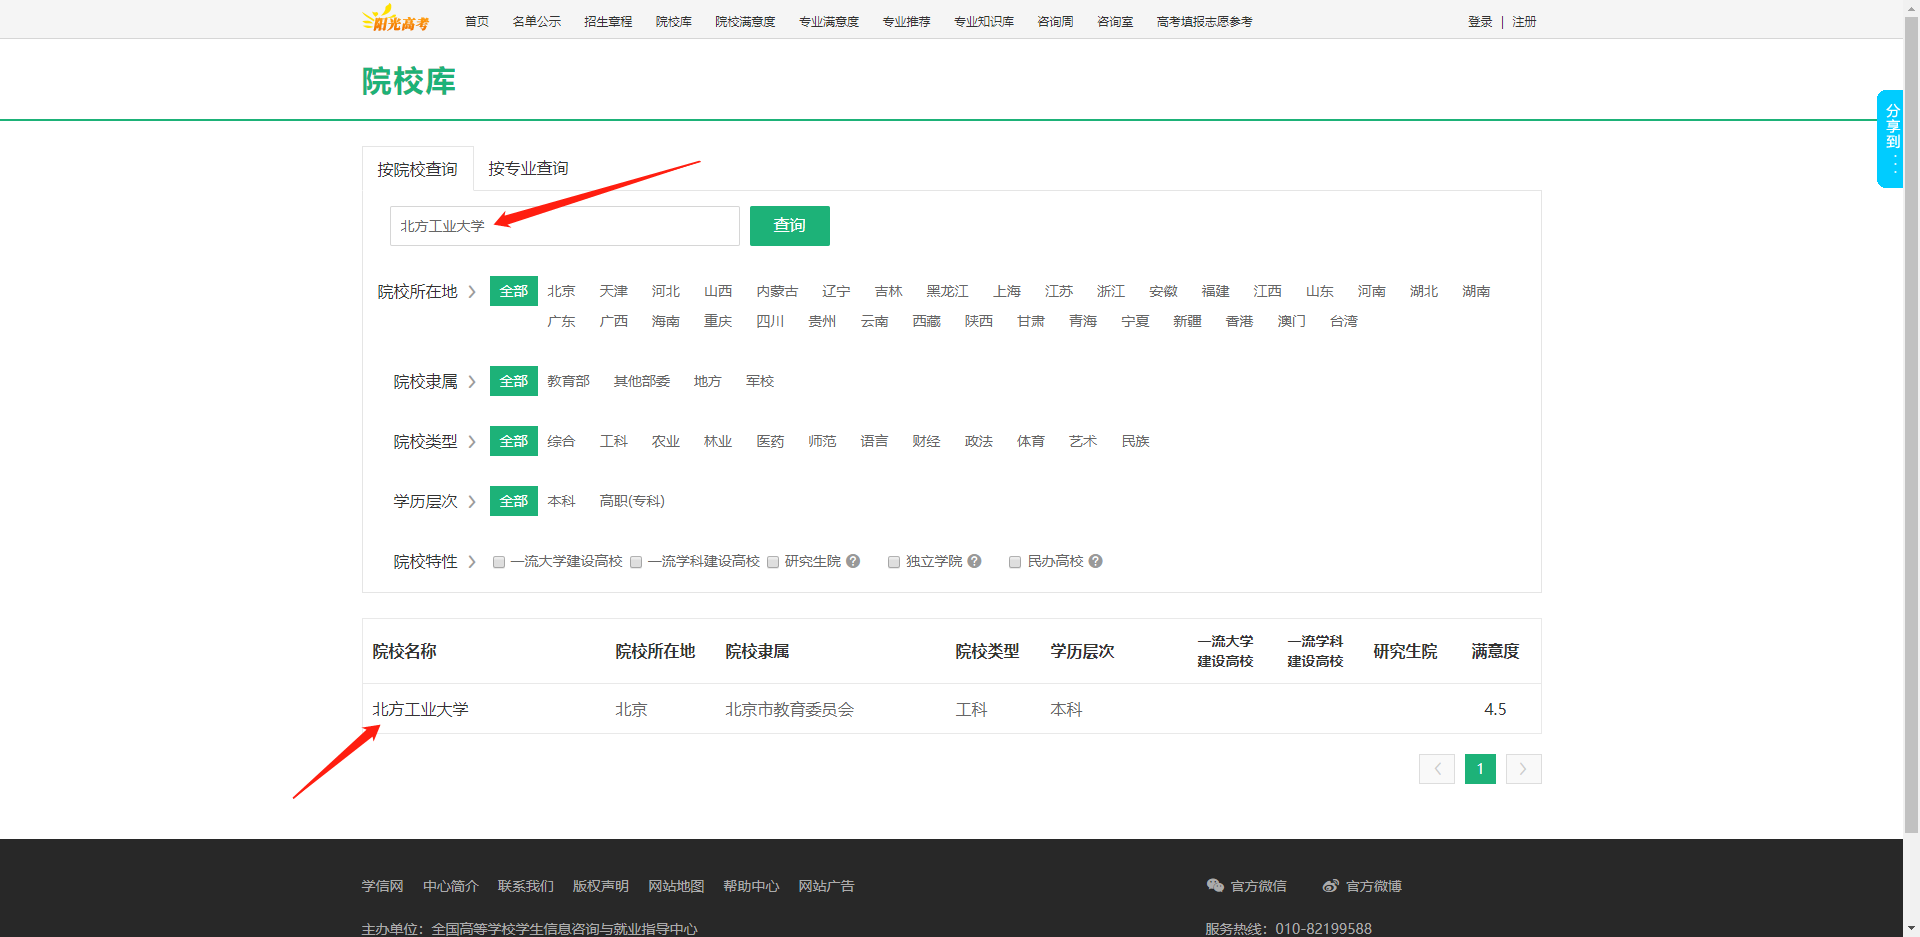
\includegraphics[width=\linewidth]{fig/search_school.png}
\caption{阳光招考网的搜索方式与搜索结果}
\end{figure}

这里用request包实现网页的下载,然后通过BeautifulSoup对html源码进行解析,并找到第一条搜索记录的网址,记录入\verb'gaokao_url'数组中。
\begin{lstlisting}
import requests
from bs4 import BeautifulSoup

gaokao_url = []
for (step,school) in enumerate(school_name,1):
  print(step,end=" ")
  url = "https://gaokao.chsi.com.cn/sch/search.do?searchType=1&yxmc=" + school + "&zymc=&sySsdm=&ssdm=&yxls=&yxlx=&xlcc="
  page = requests.get(url,timeout=30)
  soup = BeautifulSoup(page.content,'lxml')
  try:
    td = soup.find("td",attrs={"class":"js-yxk-yxmc"})
    tag = td.contents[1]
    link = tag["href"]
    gaokao_url.append("https://gaokao.chsi.com.cn" + link)
  except:
    gaokao_url.append(None)
\end{lstlisting}

\section{获取学校官网}
通过下图可以看到,在教育部招考网上,每间学校都会有对应的官网放在页面上,因此通过分析源码结构,对其中的内容进行抓取即可。
\begin{figure}[H]
\centering
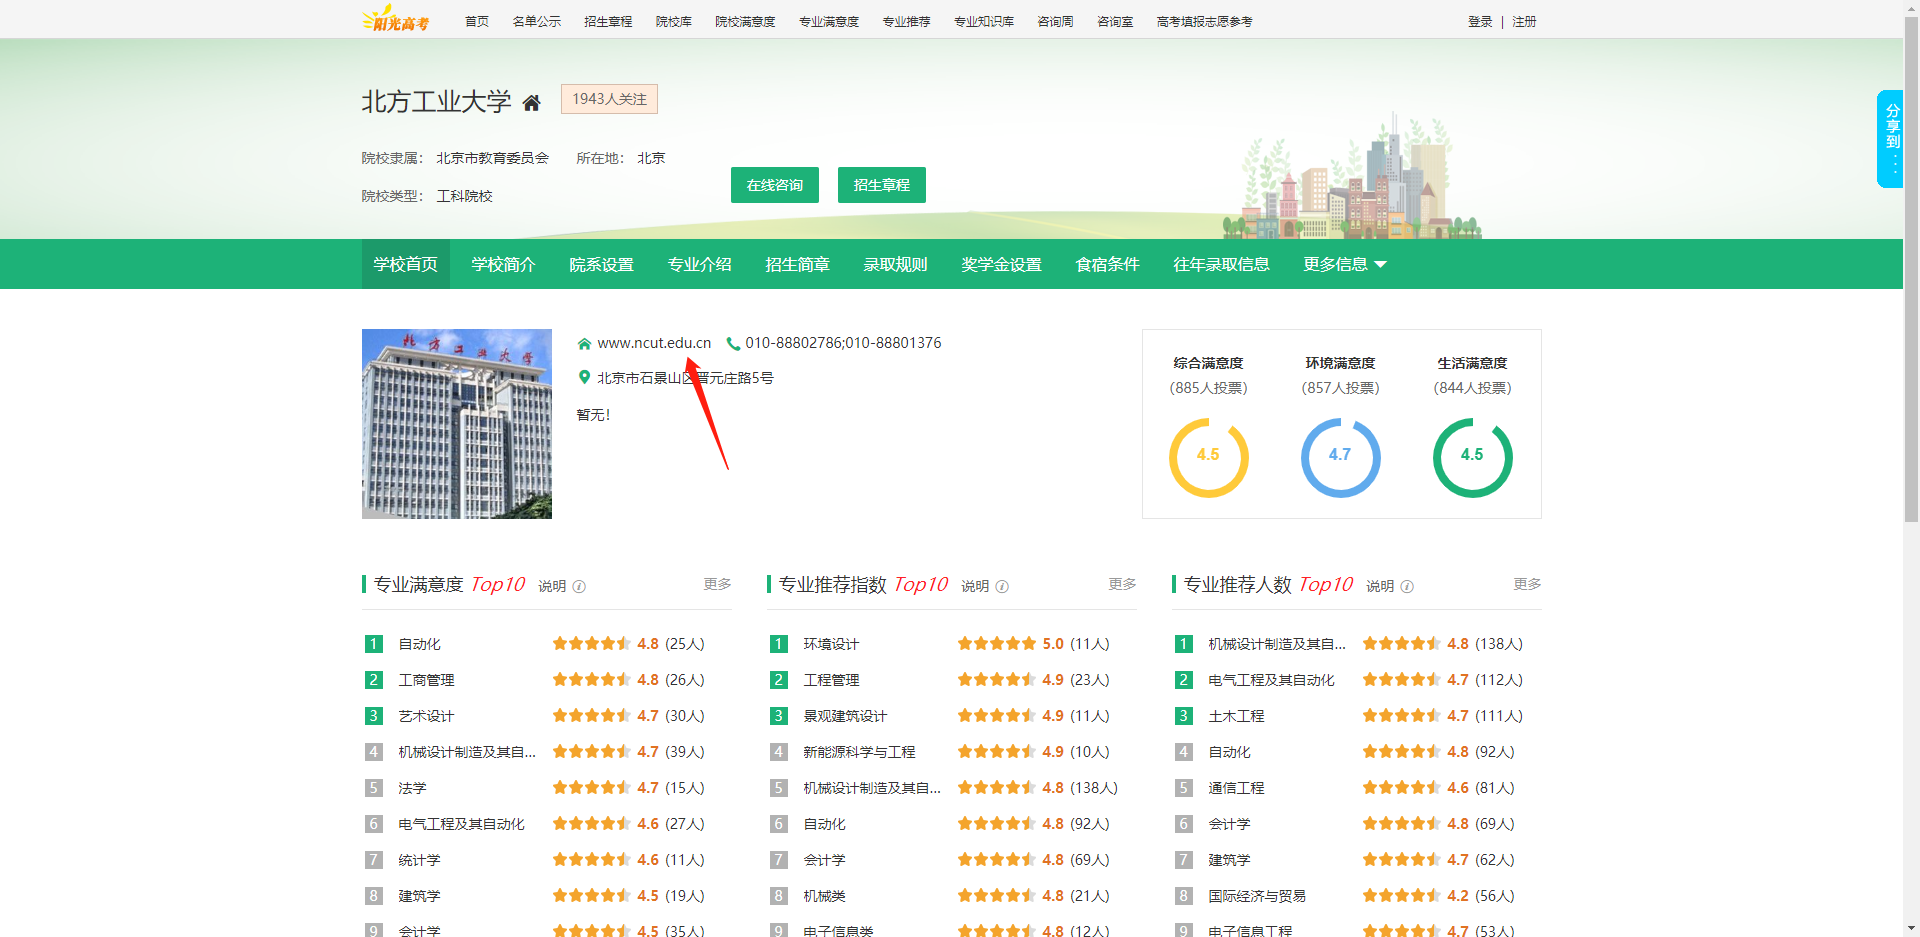
\includegraphics[width=\linewidth]{fig/get_official_url.png}
\caption{官网网址所在位置}
\end{figure}

但是这里需要注意,有些学校连教育部都没有收录其官网,这些学校我们将忽略不计。
在处理过程中则需要采用\verb'try...except...'语句来处理这种情况。
有记录官网的则将官网抓取出来加入\verb'official_url'数组中,没有记录的则直接添加\verb'None'进入数组。
同时还要注意不同页面的布局格式不太一样,因此这里有两种不同的异常处理机制。
\begin{lstlisting}
official_url = []
cnt_none = 0
for (step,url) in enumerate(gaokao_url,1):
  print(step,end=" ")
  if url == None:
    official_url.append(None)
    continue
  page = requests.get(url,timeout=30)
  soup = BeautifulSoup(page.content,'lxml')
  div = soup.find("div",attrs={"class":"msg"})
  try:
    tag = div.find("a")
    link = tag["href"]
    official_url.append(link)
  except:
    try:
      span = soup.find("span",attrs={"class":"judge-empty"})
      p = span.find("p")
      link = p.contents[0]
      official_url.append(link) # need human involution
      print(school_name[step-1],link)
    except:
      cnt_none += 1
      official_url.append(None)

print(official_url)
print(len(official_url))
outfile = open(official_url_file_name,"w")
outfile.write(str(official_url))
print(cnt_none)
\end{lstlisting}

为避免重复抓取,当所有学校官网都被抓取后,会被保存在一个文件中。
如果程序发现该文件存在,则下次运行时将直接读取,而不会再到网页上抓取,如下代码所示。
\begin{lstlisting}
if official_url_file_name not in os.listdir():
  # execute the program above
else:
  url_file = open(official_url_file_name,"r")
  official_url = eval(url_file.read())
\end{lstlisting}

\section{抓取学校网页并保存}
下面的代码则是本次实验的核心内容。

一开始我想着通过浏览器模拟来直接保存页面,即使用selenium调用Chrome的内核,并执行页面保存的操作,如下代码所示。
但是后来发现这种方式实在太过低效,因为每次调用浏览器内核都会产生巨大的运行时开销,且这些操作都是在前台运行的,对用户的其他工作非常不友好。
\begin{lstlisting}
from selenium import webdriver
from selenium.webdriver.common.action_chains import ActionChains
from selenium.webdriver.common.keys import Keys

br = webdriver.Chrome()
br.get(url)
save_me = ActionChains(br).key_down(Keys.CONTROL).key_down('s').key_up('s').key_up(Keys.CONTROL)
save_me.perform()
print("done save")
browser.implicitly_wait(5)
enter = ActionChains(br).key_down(Keys.ENTER).key_up(Keys.ENTER)
enter.perform()
\end{lstlisting}

因此后来我还是采用了最为原始的方式,即分析网页源码,从中获取内网所有页面资源并逐一进行下载,具体流程如下:
\begin{itemize}
  \item 首先抓取学校官网首页,并保存为\verb'index.html'
  \item 然后对当前网页进行html解析,从中获取所有\verb'href'标签,添加入下一级需要遍历的页面中。
  这里需要注意几点
  \begin{itemize}
    \item \verb'href'中的网页往往是相对地址,需要使用\verb'urljoin'与官网url进行整合获得绝对地址
    \item 这里判断是否学校内部网站一个简单但不一定准确的途径是看网页地址中的学校缩写是否相同,若不相同则判定为外网,在下一轮迭代中将不会对其进行分析
  \end{itemize}
  \item 不断循环遍历新页面中出现的网页(宽度优先搜索),将当前页面保存并解析链接地址。
  注意这里页面文件保存的地址与网页url的相对地址相同。
  如\verb'http:www.sysu.edu.cn\folder1\file',则\verb'file.html'将会被在\verb'www.sysu.edu.cn\foler1'的目录下,这样在本地打开离线网页时依然可以进行相对寻址。
  \item 直到不再产生新页面链接或达到最大深度时停止。(尽管进行了环检测\footnote{indexed\_url数组用于查重},但是有些学校的网站实在太过庞大,不设置最大深度根本无法爬完)
\end{itemize}
\begin{lstlisting}
import os, sys
from urllib.parse import urljoin

def crawl(pages, school_abbr, school_chinese_name, pagefolder="pages"):
  pagefolder += sep + school_chinese_name
  if not os.path.exists(pagefolder):
    os.makedirs(pagefolder)
  try:
    folder = pagefolder + sep + "index.html"
    html = requests.get(pages[0],timeout=30)
    with open(folder,"wb") as file:
      file.write(html.content)
    logger.info("Saved {}".format(folder))
  except:
    logger.info("Cannot create {}".format(folder))
    print("Cannot create {}".format(school_chinese_name))
    return

  indexed_url = []
  curr_depth = 0
  while len(pages) != 0:
    curr_depth += 1
    if curr_depth > MAX_DEPTH:
      break
    new_pages = []
    for page in pages:
      if page not in indexed_url:
        indexed_url.append(page)
        try:
          html = requests.get(page,timeout=30).content
        except:
          logger.info("Could not open {}".format(page))
          continue
        filename = page[7:].split("/")
        if filename[-1] == "" or filename[-1][-3:] == ".cn" or filename[-1][-4:] == ".com":
          folder = pagefolder + sep + filename[0]
          try:
            if not os.path.exists(folder):
              os.makedirs(folder)
            folder += sep + "index.html"
            if not os.path.isfile(folder):
              with open(folder,"wb") as file:
                file.write(html)
              logger.info("Saved {}".format(folder))
          except:
            logger.info("Cannot create {}".format(folder))
        else:
          for i,path in enumerate(filename):
            folder = pagefolder + sep + sep.join(filename[:i+1])
            if i == len(filename) - 1:
              if not os.path.isfile(folder):
                try:
                  with open(folder,"wb") as file:
                    file.write(html)
                  logger.info("Saved {}".format(folder))
                except:
                  logger.info("Cannot save {}".format(folder))
            else:
              try:
                if not os.path.exists(folder):
                  os.makedirs(folder)
              except:
                logger.info("Cannot create {}".format(folder))
        # get next urls
        soup = BeautifulSoup(html,'lxml')
        links = soup.find_all("a") # find all sub links
        for link in links:
          if "href" in dict(link.attrs):
            rel_path = link['href']
            tmp_url = urljoin(page,link['href'])
            if tmp_url.find("'") != -1 or tmp_url.find(school_abbr) == -1:
              continue
            tmp_url = tmp_url.split("#")[0]
            if tmp_url[0:4] == "http":
              new_pages.append(tmp_url)
    pages = new_pages
  print("Finish {}".format(school_abbr))
\end{lstlisting}


\section{其他设施}
\subsection{平台适应}
考虑到我的程序可能在不同的操作系统上运行,因此这里采用了platform包对操作系统进行判定。
如果发现程序运行所在的操作系统是Linux,则采用Linux的文件路径命名方式,即以\verb'/'作为分隔符;
若发现操作系统是Windows,则以\verb'\\'\footnote{这里进行了转义}作为分隔符。
\begin{lstlisting}
import platform

sep = "\\" if 'Windows' in platform.system() else "/"
\end{lstlisting}

\subsection{并发加速}
由于单核单进程进行爬虫任务的执行实在太过缓慢,因此这里采用了Python的多进程设施\footnote{之所以不使用多线程是因为Python采用了全局解释器锁(Global Interpreter Lock, GIL)机制,导致其只能使用单核CPU}来并行执行爬虫任务。

具体实施则是通过创建一个进程池\verb'Pool',然后将所有爬虫任务都添加到进程池中,交由操作系统及运行时系统进行调度。
\begin{lstlisting}
import multiprocessing

if __name__ == "__main__":
  pool = multiprocessing.Pool()
  for i in range(len(official_url)):
    url = official_url[i]
    if url == None:
      continue
    # if url == None or i < 10 or i > 20:
    #   continue
    print("Downloading {}...".format(url))
    pool.apply_async(crawl,args=([url],url.split(".")[1],str(task[i])+"-"+school_name[i]))

  pool.close()
  pool.join()
\end{lstlisting}

\subsection{日志记录}
即使开启了并发处理,爬取100所学校的网页依然是件十分耗时的工作,如果中间出现什么问题而没法跟踪的话是非常麻烦的。
因此在我的程序中采用了标准库中的\verb'logging'设施进行日志记录。
通过将重要的网页抓取信息输出到日志文件中,我就可以知道爬虫到底有没有出错,并且哪些学校的页面没有被正常抓取。
\begin{lstlisting}
import logging

logger = logging.getLogger(__name__)
logger.setLevel(level = logging.INFO)
handler = logging.FileHandler("log.txt")
handler.setLevel(logging.INFO)
formatter = logging.Formatter('%(asctime)s - %(name)s - %(levelname)s - %(message)s')
handler.setFormatter(formatter)
logger.addHandler(handler)

# example
logger.info("Saved {}".format(folder))
\end{lstlisting}

\section{实验结果}
通过分析,下面2所学院在阳光招考网上找不到对应学校,猜测学校可能更名或者被撤销了。
\begin{flushleft}
2021 广西师范学院师园学院\\
2080 海南科技职业学院
\end{flushleft}

下面3所学校则是在阳光招考网上找不到对应的学校官网,教育部网站上显示“暂无”字样。
\begin{flushleft}
1563 河南艺术职业学院\\
2546 甘肃卫生职业学院\\
2550 甘肃能源化工职业学院
\end{flushleft}

下面33所学校则无法正常访问官网\footnote{即首页都访问不了,这里抓取时采用的网络是我校的有线网。},可能是网站太久没维护,域名过期等原因导致出错。
% find . -maxdepth 1 -type d -empty
\begin{flushleft}
9 北方工业大学\\
222 河北能源职业技术学院\\
230 唐山工业职业技术学院\\
306 山西艺术职业学院\\
337 山西运城农业职业技术学院\\
433 中国刑事警察学院\\
485 沈阳职业技术学院\\
546 长春理工大学光电信息学院\\
611 哈尔滨石油学院\\
623 黑龙江职业学院\\
693 上海建桥学院\\
724 上海体育职业学院\\
809 江苏工程职业技术学院\\
829 南通科技职业学院\\
870 苏州百年职业学院\\
965 浙江艺术职业学院\\
1035  安徽信息工程学院\\
1077  安徽工商职业学院\\
1134  三明学院\\
1235  南昌工学院\\
1319  青岛农业大学\\
1403  山东外贸职业学院\\
1410  山东化工职业学院\\
1618  荆楚理工学院\\
1684  武汉科技职业学院\\
1703  湖北青年职业学院\\
1744  湖南女子学院\\
1829  湖南国防工业职业技术学院\\
1977  广东舞蹈戏剧职业学院\\
2188  四川工商学院\\
2266  安顺学院\\
2322  贵州装备制造职业学院\\
2482  陕西邮电职业技术学院
\end{flushleft}

即一共有38所高校无法获取官网网页,其余62所高校均可以正常抓取。

最终结果如下图所示,我采用学校序号+学校中文名的方式对文件夹命名,下图展示了所有95所\textbf{有官网}学校的文件夹。
\begin{figure}[H]
\centering
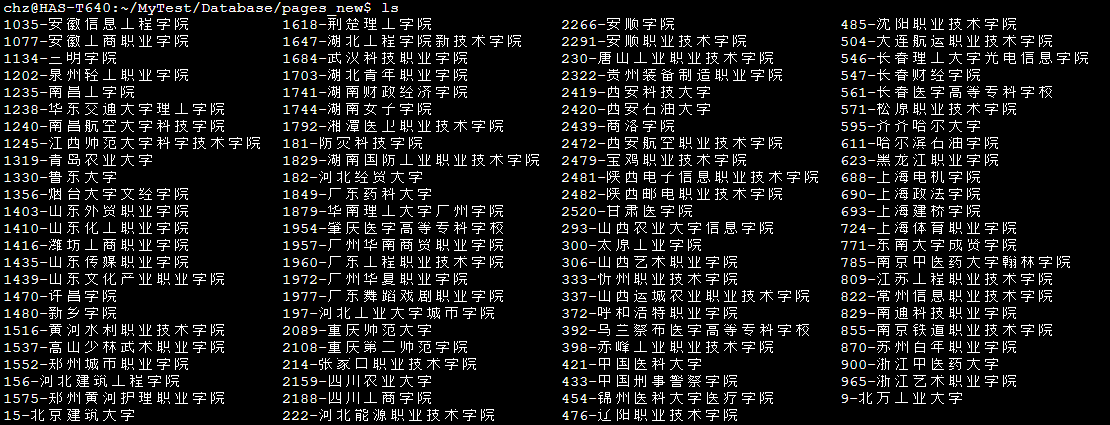
\includegraphics[width=\linewidth]{fig/all_schools.png}
\end{figure}

对于每一所学校,所有含有学校英文缩写的域名都会被抓取下来,下图是北京建筑大学的例子。
可以看到最外层会有一个名为\verb'index.html'的网页,这个即为学校官网的主页面。
其他文件夹均为与主页面同级的页面,可能是不同的学院官网,也可能是信息网页,文件夹命名方式与域名相同,方便索引。
\begin{figure}[H]
\centering
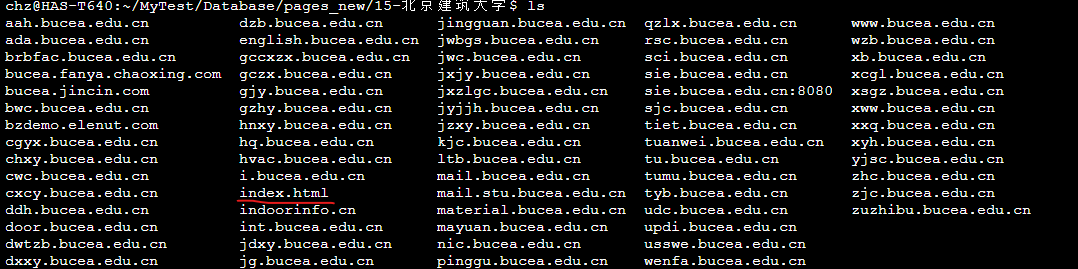
\includegraphics[width=\linewidth]{fig/eg.png}
\end{figure}

如下图所示,可以看到每个子域名下面同样是按照这种层次结构排布网页内容。
由于限制了网页抓取的深度,因此每个文件夹下的子文件夹深度也不会太大,这里仅仅是作为示意。
事实上,仅仅抓取最大深度为5的学校页面,所有学校的网页都已经达到了27G的大小。
\begin{figure}[H]
\centering
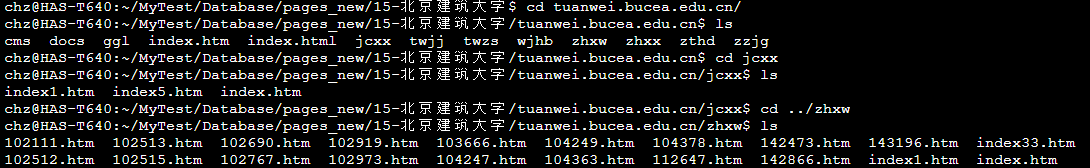
\includegraphics[width=\linewidth]{fig/eg2.png}
\end{figure}

下图是抓取下来的网页示意,可以看到页面打开后可以正常显示,仅仅包括文字内容。
如果网页中的超链接(\verb'href')采用\textbf{相对链接}的方式,则可以直接离线访问文件夹中的其他子网页,否则是无法正常跳转的,这也与各学校网页的开发人员有关。
\begin{figure}[H]
\centering
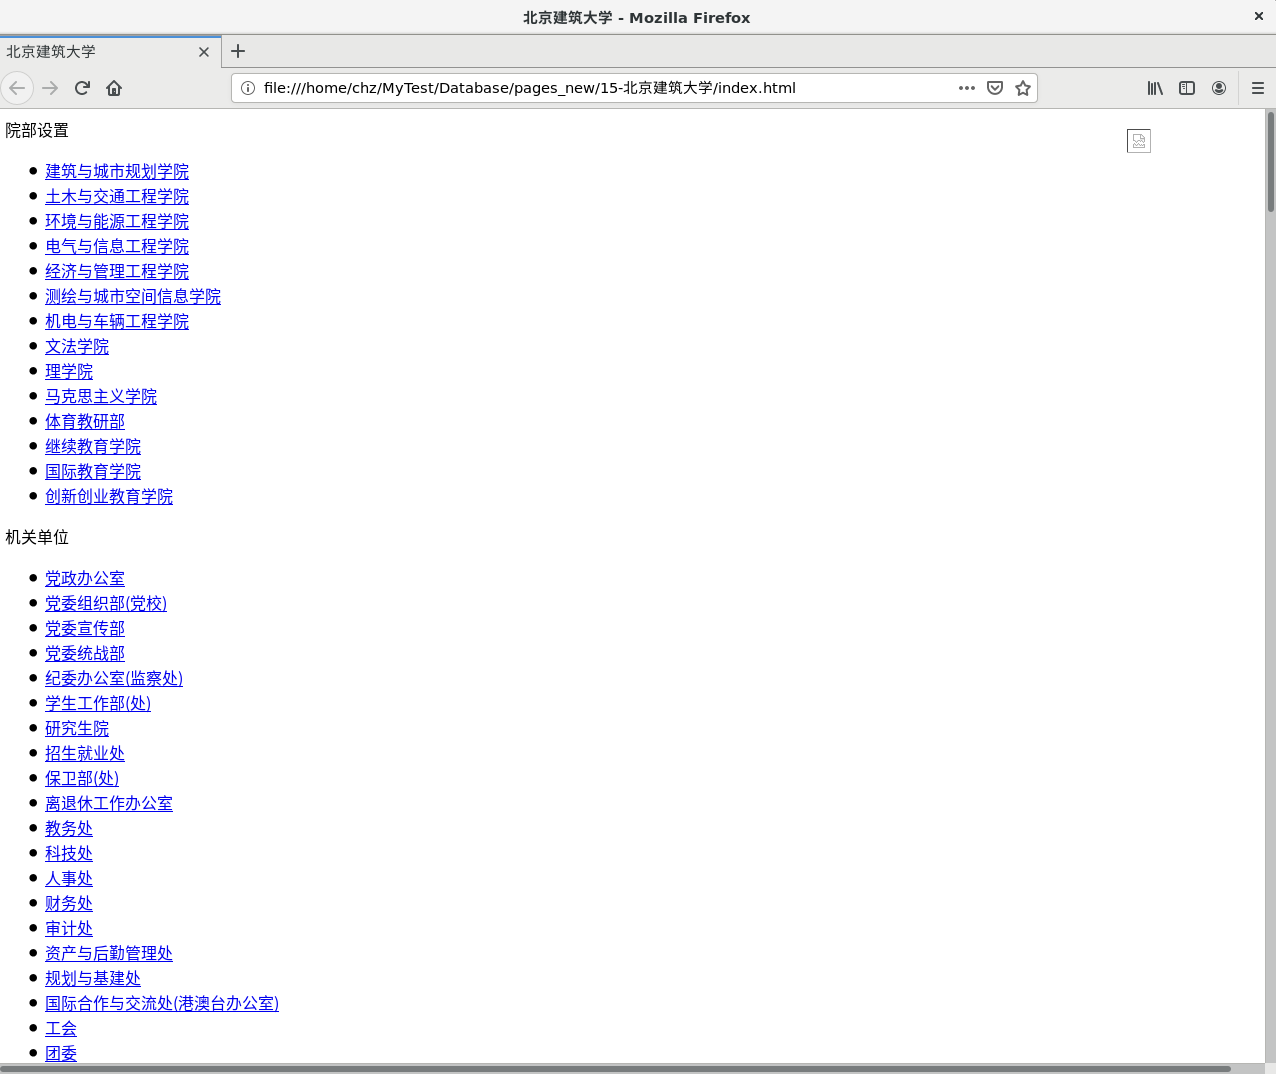
\includegraphics[width=\linewidth]{fig/eg3.png}
\end{figure}

我在每一文件目录下都创建了\verb'README.md'文档,提供说明帮助,一个例子如下。
由于采用了python元语言方式生成,因此每间学校的说明文档也是不一样的。
\begin{figure}[H]
\centering
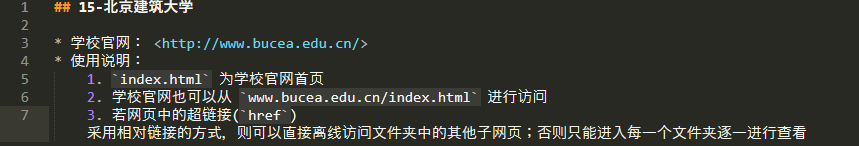
\includegraphics[width=\linewidth]{fig/readme.png}
\end{figure}

所有中间结果文件也都附在附件中,可以查阅。

\appendixconfig
\appendix
\section{学校名称及官网对应}
\label{app:school}
\begin{longtable}{|l|l|l|}
\hline
序号 & 学校名称 & 学校官网\\\hline
9 & 北方工业大学 & \url{http://www.ncut.edu.cn/}\\\hline
15 & 北京建筑大学 & \url{http://www.bucea.edu.cn/}\\\hline
156 & 河北建筑工程学院 & \url{http://www.hebiace.edu.cn/}\\\hline
181 & 防灾科技学院 & \url{http://www.cidp.edu.cn}\\\hline
182 & 河北经贸大学 & \url{http://www.heuet.edu.cn/}\\\hline
197 & 河北工业大学城市学院 & \url{http://cc.hebut.edu.cn/}\\\hline
214 & 张家口职业技术学院 & \url{http://www.zhz.cn/}\\\hline
222 & 河北能源职业技术学院 & \url{http://www.hbnyxy.cn/}\\\hline
230 & 唐山工业职业技术学院 & \url{http://www.tsgzy.edu.cn/}\\\hline
293 & 山西农业大学信息学院 & \url{http://www.cisau.com.cn/}\\\hline
300 & 太原工业学院 & \url{http://www.tit.edu.cn/}\\\hline
306 & 山西艺术职业学院 & \url{http://www.sxyz.com/}\\\hline
333 & 忻州职业技术学院 & \url{http://www.xzvtc.com/}\\\hline
337 & 山西运城农业职业技术学院 & \url{http://www.ycnxy.com/}\\\hline
372 & 呼和浩特职业学院 & \url{http://www.hhvc.edu.cn/}\\\hline
392 & 乌兰察布医学高等专科学校 & \url{http://www.wlcbyz.org.cn}\\\hline
398 & 赤峰工业职业技术学院 & \url{http://www.nmgfzxx.cn/}\\\hline
421 & 中国医科大学 & \url{http://www.cmu.edu.cn/}\\\hline
433 & 中国刑事警察学院 & \url{http://www.cipuc.edu.cn}\\\hline
454 & 锦州医科大学医疗学院 & \url{http://www.jymu.edu.cn}\\\hline
476 & 辽阳职业技术学院 & \url{http://www.419.com.cn/}\\\hline
485 & 沈阳职业技术学院 & \url{http://www.vtcsy.com/}\\\hline
504 & 大连航运职业技术学院 & \url{http://www.dlsc.net.cn/}\\\hline
546 & 长春理工大学光电信息学院 & \url{http://www.csoei.com/}\\\hline
547 & 长春财经学院 & \url{http://www.ccufe.com/}\\\hline
561 & 长春医学高等专科学校 & \url{http://www.ccmc.edu.cn/}\\\hline
571 & 松原职业技术学院 & \url{http://www.sypt.cn/}\\\hline
595 & 齐齐哈尔大学 & \url{http://www.qqhru.edu.cn/}\\\hline
611 & 哈尔滨石油学院 & \url{http://www.hip.edu.cn/}\\\hline
623 & 黑龙江职业学院 & \url{http://www.hljp.edu.cn}\\\hline
688 & 上海电机学院 & \url{http://www.sdju.edu.cn/}\\\hline
690 & 上海政法学院 & \url{http://www.shupl.edu.cn}\\\hline
693 & 上海建桥学院 & \url{http://61.172.146.40/}\\\hline
724 & 上海体育职业学院 & \url{http://www.ssi.edu.cn/}\\\hline
771 & 东南大学成贤学院 & \url{http://cxxy.seu.edu.cn/}\\\hline
785 & 南京中医药大学翰林学院 & \url{http://www.hlxy.edu.cn/}\\\hline
809 & 江苏工程职业技术学院 & \url{http://www.jcet.edu.cn/}\\\hline
822 & 常州信息职业技术学院 & \url{http://zjczs.ccit.js.cn/}\\\hline
829 & 南通科技职业学院 & \url{http://www.ntac.edu.cn/}\\\hline
855 & 南京铁道职业技术学院 & \url{http://www.njrts.edu.cn/}\\\hline
870 & 苏州百年职业学院 & \url{http://www.hkuspace.edu.cn/}\\\hline
900 & 浙江中医药大学 & \url{http://www.zcmu.edu.cn}\\\hline
965 & 浙江艺术职业学院 & \url{http://zhaosheng.zj-art.com/}\\\hline
1035 & 安徽信息工程学院 & \url{http://www.ahpumec.edu.cn/}\\\hline
1077 & 安徽工商职业学院 & \url{http://ahbvc.cn/}\\\hline
1134 & 三明学院 & \url{mailto:smxyzsb@163.com}\\\hline
1202 & 泉州轻工职业学院 & \url{http://www.qzqgxy.com/}\\\hline
1235 & 南昌工学院 & \url{http://www.ncpu.edu.cn}\\\hline
1238 & 华东交通大学理工学院 & \url{http://www.ecjtuit.com.cn/}\\\hline
1240 & 南昌航空大学科技学院 & \url{http://www.nckjxy.cn/}\\\hline
1245 & 江西师范大学科学技术学院 & \url{http://kjxy.jxnu.edu.cn/}\\\hline
1319 & 青岛农业大学 & \url{http://www.qau.edu.cn/}\\\hline
1330 & 鲁东大学 & \url{http://www.ldu.edu.cn/}\\\hline
1356 & 烟台大学文经学院 & \url{http://wenjing.ytu.edu.cn/}\\\hline
1403 & 山东外贸职业学院 & \url{http://www.sdwm.cn}\\\hline
1410 & 山东化工职业学院 & \url{http://www.qledu.net/}\\\hline
1416 & 潍坊工商职业学院 & \url{http://www.wfgsxy.com/}\\\hline
1435 & 山东传媒职业学院 & \url{http://www.sdcmc.net/}\\\hline
1439 & 山东文化产业职业学院 & \url{http://www.sdcivc.com/}\\\hline
1470 & 许昌学院 & \url{http://www.xcu.edu.cn/}\\\hline
1480 & 新乡学院 & \url{http://www.xxu.edu.cn}\\\hline
1516 & 黄河水利职业技术学院 & \url{http://www.yrcti.edu.cn}\\\hline
1537 & 嵩山少林武术职业学院 & \url{http://www.shaolinkungfu.edu.cn/}\\\hline
1552 & 郑州城市职业学院 & \url{http://www.zcu.edu.cn/}\\\hline
1563 & 河南艺术职业学院 & None\\\hline
1575 & 郑州黄河护理职业学院 & \url{http://www.zyrnvc.com/}\\\hline
1618 & 荆楚理工学院 & \url{http://www.jcut.edu.cn/}\\\hline
1647 & 湖北工程学院新技术学院 & \url{http://www.hbeutc.cn}\\\hline
1684 & 武汉科技职业学院 & \url{http://www.whuvt.com}\\\hline
1703 & 湖北青年职业学院 & \url{http://www.hbqnxy.com/}\\\hline
1741 & 湖南财政经济学院 & \url{http://www.hufe.edu.cn/}\\\hline
1744 & 湖南女子学院 & \url{http://www.hnwu.edu.cn/}\\\hline
1792 & 湘潭医卫职业技术学院 & \url{http://www.xtzy.com}\\\hline
1829 & 湖南国防工业职业技术学院 & \url{http://www.hnkgzy.com/}\\\hline
1849 & 广东药科大学 & \url{http://www.gdpu.edu.cn/}\\\hline
1879 & 华南理工大学广州学院 & \url{http://www.gcu.edu.cn/}\\\hline
1954 & 肇庆医学高等专科学校 & \url{http://www.zqyz.gd.cn/}\\\hline
1957 & 广州华南商贸职业学院 & \url{http://www.hnsmxy.com/}\\\hline
1960 & 广东工程职业技术学院 & \url{http://www.gpc.net.cn/}\\\hline
1972 & 广州华夏职业学院 & \url{http://www.gzhxtc.cn/}\\\hline
1977 & 广东舞蹈戏剧职业学院 & \url{http://www.gdddc.cn}\\\hline
2021 & 广西师范学院师园学院 & None\\\hline
2080 & 海南科技职业学院 & None\\\hline
2089 & 重庆师范大学 & \url{http://www.cqnu.edu.cn/}\\\hline
2108 & 重庆第二师范学院 & \url{http://www.cque.edu.cn}\\\hline
2159 & 四川农业大学 & \url{http://www.sicau.edu.cn/}\\\hline
2188 & 四川工商学院 & \url{http://www.cdxy.edu.cn/}\\\hline
2266 & 安顺学院 & \url{http://www.asu.edu.cn/}\\\hline
2291 & 安顺职业技术学院 & \url{http://www.asotc.cn/}\\\hline
2322 & 贵州装备制造职业学院 & \url{http://www.gzzbzy.cn}\\\hline
2419 & 西安科技大学 & \url{http://www.xust.edu.cn}\\\hline
2420 & 西安石油大学 & \url{http://www.xsyu.edu.cn/}\\\hline
2439 & 商洛学院 & \url{http://www.slxy.cn/}\\\hline
2472 & 西安航空职业技术学院 & \url{http://www.xihang.com.cn/}\\\hline
2479 & 宝鸡职业技术学院 & \url{http://www.bjvtc.com/}\\\hline
2481 & 陕西电子信息职业技术学院 & \url{http://www.sxitu.com/}\\\hline
2482 & 陕西邮电职业技术学院 & \url{http://www.sptc.sn.cn/}\\\hline
2520 & 甘肃医学院 & \url{http://www.plmc.edu.cn/}\\\hline
2546 & 甘肃卫生职业学院 & None\\\hline
2550 & 甘肃能源化工职业学院 & None\\\hline
\end{longtable}

\section{附件说明}
\begin{itemize}
  \item \verb'spider':爬虫核心程序
  \item \verb'analysis':网页爬取后分析及\verb'README.md'写入
  \item \verb'all_school_url':附录\ref{app:school}
  \item \verb'gaokao_url':阳光招考网上对应网站
  \item \verb'official_url_new':学校官网数组
  \item \verb'school_chinese':学校中文名数组
  \item \verb'log.txt':程序运行日志
\end{itemize}
% tar cf - pages_new -P | pv -s $(du -sb pages_new | awk '{print $1}') | gzip --best > 17341015_pages.tar.gz

\end{document}

% 截止时间: 2019-10-09 23:59:59
% 每个同学会被分配100个高校,抓取这些高校官网发布的信息
% 要求:
% * 尽可能把该网站中所有公开内容(可以排除图片, 样式,js脚本)抓取下来,不限层级
% * 网页内容要统一以utf8编码保存
% * 抓取的页面内容与页面链接需要一一对应,同一个链接只要保存一个页面
% * 将源码、抓取的内容、对应的链接以及一份简单的说明文档(说明如何将你的链接与内容对应)打包压缩并上传到百度云盘,并写一份报告,主要讲述遇到的问题以及自己如何解决。
%   * 源码+数据,与报告分开上传到相应的文件夹,命名规则为 学号_姓名_实验主题.doc/zip...